 \documentclass[oneside,a4paper,12pt]{book}
%\pagestyle{headings}
\frontmatter

% !TEX encoding = UTF-8 Unicode

%=============================================================================

% Just add % !TEX encoding = UTF-8 Unicode

%=============================================================================

% Just add % !TEX encoding = UTF-8 Unicode

%=============================================================================

% Just add \input{smalltalkEnv} to your file
% then you can use :
% \begin{lstlisting}[language=Smalltalk]
% false become: true.
% \end{lstlisting}


\usepackage{color}
\usepackage{listings}
\usepackage{etoolbox}
\usepackage{textcomp}
\usepackage{xpatch}
\usepackage{tcolorbox}

\definecolor{source}{gray}{0.95}

\definecolor{stComment}{rgb}{0.5,0.5,0.5}
\definecolor{stString}{rgb}{0.58,0,0.82}
\definecolor{stKeywords}{rgb}{0.21,0.55,0.7}
\definecolor{stNumbers}{rgb}{.5,0,0}

\newtoggle{InString}{}% Keep track of if we are within a string
\togglefalse{InString}% Assume not initally in string
\newcommand*{\ColorIfNotInString}[1]{\iftoggle{InString}{#1}{\color{stNumbers}#1}}%
\newcommand*{\ProcessQuote}[1]{#1\iftoggle{InString}{\global\togglefalse{InString}}{\global\toggletrue{InString}}}%

\lstdefinelanguage{Smalltalk}{
  basicstyle=\sffamily\scriptsize,
  keywordstyle=\color{stKeywords},
  commentstyle=\color{stComment},
  stringstyle=\color{stString},
  alsoletter=\#,
  identifierstyle=\idstyle, 
  showstringspaces=false,
  morekeywords={true,false,self,super,nil},
  backgroundcolor=\color{source},
  sensitive=true, 
  morecomment=[s]{"}{"}, 
  morestring=[d]', 
  style=SmalltalkStyle,
  literate=
    {BANG}{!}1
    {UNDERSCORE}{\_}1
    {\\st}{Smalltalk}9 % convenience -- in case \st occurs in code
    % {'}{{\textquotesingle}}1 % replaced by upquote=true in \lstset
    {_}{{$\leftarrow$}}1
    {>>>}{{\sep}}1
    {^}{{$\uparrow$}}1
    {~}{{$\sim$}}1
    {-}{{\sf -\hspace{-0.13em}-}}1  % the goal is to make - the same width as +
    {+}{\raisebox{0.08ex}{+}}1		% and to raise + off the baseline to match -
    {-->}{{\quad$\longrightarrow$\quad}}3
	, % Don't forget the comma at the end!
  tabsize=2,
}



\makeatletter%
\newcommand*\idstyle[1]{%
  \expandafter\id@style\the\lst@token{#1}\relax%
}
\def\id@style#1#2\relax{%
  \ifnum\pdfstrcmp{#1}{\#}=0%
  \color{stString} \the\lst@token%
  \else%
  \edef\tempa{\uccode`#1}%
  \edef\tempb{`#1}%
  \ifnum\tempa=\tempb%
  \color{blue} \the\lst@token%
  \else%
  \the\lst@token%
  \fi%
  \fi%
}

\lstdefinestyle{SmalltalkStyle}{ 
  literate=%
  {^}{{$\uparrow$}}1% 
  % {"}{{{\ProcessQuote{"}}}}1% Disable coloring within double quotes
  % {'}{{{\ProcessQuote{'}}}}1% Disable coloring within single quote
  {0}{{{\ColorIfNotInString{0}}}}1%
  {1}{{{\ColorIfNotInString{1}}}}1%
  {2}{{{\ColorIfNotInString{2}}}}1%
  {3}{{{\ColorIfNotInString{3}}}}1%
  {4}{{{\ColorIfNotInString{4}}}}1%
  {5}{{{\ColorIfNotInString{5}}}}1%
  {6}{{{\ColorIfNotInString{6}}}}1%
  {7}{{{\ColorIfNotInString{7}}}}1%
  {8}{{{\ColorIfNotInString{8}}}}1%
  {9}{{{\ColorIfNotInString{9}}}}1%
} 

\lstset{% setup listings
    framexleftmargin=6pt,
    framextopmargin=6pt,
    framexbottommargin=6pt, 
    frame=tb, framerule=0pt,
}


% In-line code (literal)  with background color
% Normally use this for all in-line code:
\newcommand{\ct}[1]{{\colorbox{source}{\lstinline[mathescape=false,backgroundcolor=\color{source},basicstyle={\sffamily\small}]{#1}}}}


% In-line code (latex enabled)
% Use this only in special situations where \ct does not work
% (within section headings ...):
\newcommand{\lct}[1]{{\textsf{\textup{#1}}}}
% Code environments
\lstnewenvironment{code}{%
	\lstset{%
	    escapeinside={(*@}{@*)},
		% frame=lines,
		frame=single,
		framerule=0pt,
		mathescape=false
	}%
}{%
}


\newcommand*\DNumber{\addtocounter{lstnumber}{-1}}
%%% Always I forget this so I created some aliases
\def\ContinueLineNumber{\lstset{firstnumber=last}}
\def\StartLineAt#1{\lstset{firstnumber=#1}}
\let\numberLineAt\StartLineAt to your file
% then you can use :
% \begin{lstlisting}[language=Smalltalk]
% false become: true.
% \end{lstlisting}


\usepackage{color}
\usepackage{listings}
\usepackage{etoolbox}
\usepackage{textcomp}
\usepackage{xpatch}
\usepackage{tcolorbox}

\definecolor{source}{gray}{0.95}

\definecolor{stComment}{rgb}{0.5,0.5,0.5}
\definecolor{stString}{rgb}{0.58,0,0.82}
\definecolor{stKeywords}{rgb}{0.21,0.55,0.7}
\definecolor{stNumbers}{rgb}{.5,0,0}

\newtoggle{InString}{}% Keep track of if we are within a string
\togglefalse{InString}% Assume not initally in string
\newcommand*{\ColorIfNotInString}[1]{\iftoggle{InString}{#1}{\color{stNumbers}#1}}%
\newcommand*{\ProcessQuote}[1]{#1\iftoggle{InString}{\global\togglefalse{InString}}{\global\toggletrue{InString}}}%

\lstdefinelanguage{Smalltalk}{
  basicstyle=\sffamily\scriptsize,
  keywordstyle=\color{stKeywords},
  commentstyle=\color{stComment},
  stringstyle=\color{stString},
  alsoletter=\#,
  identifierstyle=\idstyle, 
  showstringspaces=false,
  morekeywords={true,false,self,super,nil},
  backgroundcolor=\color{source},
  sensitive=true, 
  morecomment=[s]{"}{"}, 
  morestring=[d]', 
  style=SmalltalkStyle,
  literate=
    {BANG}{!}1
    {UNDERSCORE}{\_}1
    {\\st}{Smalltalk}9 % convenience -- in case \st occurs in code
    % {'}{{\textquotesingle}}1 % replaced by upquote=true in \lstset
    {_}{{$\leftarrow$}}1
    {>>>}{{\sep}}1
    {^}{{$\uparrow$}}1
    {~}{{$\sim$}}1
    {-}{{\sf -\hspace{-0.13em}-}}1  % the goal is to make - the same width as +
    {+}{\raisebox{0.08ex}{+}}1		% and to raise + off the baseline to match -
    {-->}{{\quad$\longrightarrow$\quad}}3
	, % Don't forget the comma at the end!
  tabsize=2,
}



\makeatletter%
\newcommand*\idstyle[1]{%
  \expandafter\id@style\the\lst@token{#1}\relax%
}
\def\id@style#1#2\relax{%
  \ifnum\pdfstrcmp{#1}{\#}=0%
  \color{stString} \the\lst@token%
  \else%
  \edef\tempa{\uccode`#1}%
  \edef\tempb{`#1}%
  \ifnum\tempa=\tempb%
  \color{blue} \the\lst@token%
  \else%
  \the\lst@token%
  \fi%
  \fi%
}

\lstdefinestyle{SmalltalkStyle}{ 
  literate=%
  {^}{{$\uparrow$}}1% 
  % {"}{{{\ProcessQuote{"}}}}1% Disable coloring within double quotes
  % {'}{{{\ProcessQuote{'}}}}1% Disable coloring within single quote
  {0}{{{\ColorIfNotInString{0}}}}1%
  {1}{{{\ColorIfNotInString{1}}}}1%
  {2}{{{\ColorIfNotInString{2}}}}1%
  {3}{{{\ColorIfNotInString{3}}}}1%
  {4}{{{\ColorIfNotInString{4}}}}1%
  {5}{{{\ColorIfNotInString{5}}}}1%
  {6}{{{\ColorIfNotInString{6}}}}1%
  {7}{{{\ColorIfNotInString{7}}}}1%
  {8}{{{\ColorIfNotInString{8}}}}1%
  {9}{{{\ColorIfNotInString{9}}}}1%
} 

\lstset{% setup listings
    framexleftmargin=6pt,
    framextopmargin=6pt,
    framexbottommargin=6pt, 
    frame=tb, framerule=0pt,
}


% In-line code (literal)  with background color
% Normally use this for all in-line code:
\newcommand{\ct}[1]{{\colorbox{source}{\lstinline[mathescape=false,backgroundcolor=\color{source},basicstyle={\sffamily\small}]{#1}}}}


% In-line code (latex enabled)
% Use this only in special situations where \ct does not work
% (within section headings ...):
\newcommand{\lct}[1]{{\textsf{\textup{#1}}}}
% Code environments
\lstnewenvironment{code}{%
	\lstset{%
	    escapeinside={(*@}{@*)},
		% frame=lines,
		frame=single,
		framerule=0pt,
		mathescape=false
	}%
}{%
}


\newcommand*\DNumber{\addtocounter{lstnumber}{-1}}
%%% Always I forget this so I created some aliases
\def\ContinueLineNumber{\lstset{firstnumber=last}}
\def\StartLineAt#1{\lstset{firstnumber=#1}}
\let\numberLineAt\StartLineAt to your file
% then you can use :
% \begin{lstlisting}[language=Smalltalk]
% false become: true.
% \end{lstlisting}


\usepackage{color}
\usepackage{listings}
\usepackage{etoolbox}
\usepackage{textcomp}
\usepackage{xpatch}
\usepackage{tcolorbox}

\definecolor{source}{gray}{0.95}

\definecolor{stComment}{rgb}{0.5,0.5,0.5}
\definecolor{stString}{rgb}{0.58,0,0.82}
\definecolor{stKeywords}{rgb}{0.21,0.55,0.7}
\definecolor{stNumbers}{rgb}{.5,0,0}

\newtoggle{InString}{}% Keep track of if we are within a string
\togglefalse{InString}% Assume not initally in string
\newcommand*{\ColorIfNotInString}[1]{\iftoggle{InString}{#1}{\color{stNumbers}#1}}%
\newcommand*{\ProcessQuote}[1]{#1\iftoggle{InString}{\global\togglefalse{InString}}{\global\toggletrue{InString}}}%

\lstdefinelanguage{Smalltalk}{
  basicstyle=\sffamily\scriptsize,
  keywordstyle=\color{stKeywords},
  commentstyle=\color{stComment},
  stringstyle=\color{stString},
  alsoletter=\#,
  identifierstyle=\idstyle, 
  showstringspaces=false,
  morekeywords={true,false,self,super,nil},
  backgroundcolor=\color{source},
  sensitive=true, 
  morecomment=[s]{"}{"}, 
  morestring=[d]', 
  style=SmalltalkStyle,
  literate=
    {BANG}{!}1
    {UNDERSCORE}{\_}1
    {\\st}{Smalltalk}9 % convenience -- in case \st occurs in code
    % {'}{{\textquotesingle}}1 % replaced by upquote=true in \lstset
    {_}{{$\leftarrow$}}1
    {>>>}{{\sep}}1
    {^}{{$\uparrow$}}1
    {~}{{$\sim$}}1
    {-}{{\sf -\hspace{-0.13em}-}}1  % the goal is to make - the same width as +
    {+}{\raisebox{0.08ex}{+}}1		% and to raise + off the baseline to match -
    {-->}{{\quad$\longrightarrow$\quad}}3
	, % Don't forget the comma at the end!
  tabsize=2,
}



\makeatletter%
\newcommand*\idstyle[1]{%
  \expandafter\id@style\the\lst@token{#1}\relax%
}
\def\id@style#1#2\relax{%
  \ifnum\pdfstrcmp{#1}{\#}=0%
  \color{stString} \the\lst@token%
  \else%
  \edef\tempa{\uccode`#1}%
  \edef\tempb{`#1}%
  \ifnum\tempa=\tempb%
  \color{blue} \the\lst@token%
  \else%
  \the\lst@token%
  \fi%
  \fi%
}

\lstdefinestyle{SmalltalkStyle}{ 
  literate=%
  {^}{{$\uparrow$}}1% 
  % {"}{{{\ProcessQuote{"}}}}1% Disable coloring within double quotes
  % {'}{{{\ProcessQuote{'}}}}1% Disable coloring within single quote
  {0}{{{\ColorIfNotInString{0}}}}1%
  {1}{{{\ColorIfNotInString{1}}}}1%
  {2}{{{\ColorIfNotInString{2}}}}1%
  {3}{{{\ColorIfNotInString{3}}}}1%
  {4}{{{\ColorIfNotInString{4}}}}1%
  {5}{{{\ColorIfNotInString{5}}}}1%
  {6}{{{\ColorIfNotInString{6}}}}1%
  {7}{{{\ColorIfNotInString{7}}}}1%
  {8}{{{\ColorIfNotInString{8}}}}1%
  {9}{{{\ColorIfNotInString{9}}}}1%
} 

\lstset{% setup listings
    framexleftmargin=6pt,
    framextopmargin=6pt,
    framexbottommargin=6pt, 
    frame=tb, framerule=0pt,
}


% In-line code (literal)  with background color
% Normally use this for all in-line code:
\newcommand{\ct}[1]{{\colorbox{source}{\lstinline[mathescape=false,backgroundcolor=\color{source},basicstyle={\sffamily\small}]{#1}}}}


% In-line code (latex enabled)
% Use this only in special situations where \ct does not work
% (within section headings ...):
\newcommand{\lct}[1]{{\textsf{\textup{#1}}}}
% Code environments
\lstnewenvironment{code}{%
	\lstset{%
	    escapeinside={(*@}{@*)},
		% frame=lines,
		frame=single,
		framerule=0pt,
		mathescape=false
	}%
}{%
}


\newcommand*\DNumber{\addtocounter{lstnumber}{-1}}
%%% Always I forget this so I created some aliases
\def\ContinueLineNumber{\lstset{firstnumber=last}}
\def\StartLineAt#1{\lstset{firstnumber=#1}}
\let\numberLineAt\StartLineAt
% !TEX encoding = UTF-8 Unicode

%=============================================================================

\usepackage{amsthm}
\usepackage{xspace}
\usepackage{float}
\usepackage{ifthen}
\usepackage{amsbsy}
\usepackage{amssymb}
\usepackage{balance}
\usepackage{booktabs}
\usepackage{graphicx}
\usepackage{rotating}
\usepackage{multirow}
\usepackage{needspace}
\usepackage{microtype}
\usepackage{bold-extra}
\usepackage{geometry}
\usepackage{varioref}
\usepackage{xcolor}
\usepackage{textcomp}
\usepackage{listings}
\usepackage[normalem]{ulem} %emphasize still italic
\usepackage{ucs}
\usepackage{csquotes}

\usepackage[utf8]{inputenc}
% \usepackage[htt]{hyphenat}
\usepackage{times}
\usepackage{url}
\usepackage{alltt}
\usepackage{amsmath}
\usepackage{xfrac}
\usepackage{subfig}
\usepackage{appendix}
\usepackage{stmaryrd}   % for the \shortuparrow
\usepackage[utopia]{quotchap}

\usepackage{setspace}
\usepackage[numbers, sort&compress]{natbib}
\usepackage{mdwlist}        % support for better spaced lists
% allows for temporary adjustment of side margins
\usepackage{chngpage}
\usepackage[normalem]{ulem} 

% constants

\newcounter{qcounter}

% commands
\newcommand{\n}{$\cdot$}
\newcommand{\y}{\checkmark}
\newcommand{\subscript}[1]{$_{\textrm{\footnotesize{#1}}}$}
\newcommand{\superscript}[1]{$^{\textrm{\footnotesize{#1}}}$}
\newcommand{\vertical}[1]{\raisebox{-4em}{\begin{sideways}{#1}\end{sideways}}}

\newboolean{showedits}
\setboolean{showedits}{true} % toggle to show or hide edits
\ifthenelse{\boolean{showedits}}
{
       \newcommand{\ugh}[1]{\textcolor{red}{\uwave{#1}}} % please rephrase
       \newcommand{\ins}[1]{\textcolor{blue}{\uline{#1}}} % please insert
       \newcommand{\del}[1]{\textcolor{red}{\sout{#1}}} % please delete
       \newcommand{\chg}[2]{\textcolor{red}{\sout{#1}}{\ra}\textcolor{blue}{\uline{#2}}} % please change
}{
       \newcommand{\ugh}[1]{#1} % please rephrase
       \newcommand{\ins}[1]{#1} % please insert
       \newcommand{\del}[1]{} % please delete
       \newcommand{\chg}[2]{#2}
}


% ============================================================================
% Put edit comments in a really ugly standout display

\usepackage{xcolor}
\usepackage[normalem]{ulem}
\newcommand{\ra}{$\rightarrow$}


% comments \nb{label}{color}{text}
\newboolean{showcomments}
\setboolean{showcomments}{true}
\ifthenelse{\boolean{showcomments}}
    {\newcommand{\nb}[3]{
        {\colorbox{#2}{\bfseries\sffamily\scriptsize\textcolor{white}{#1}}}
        {\textcolor{#2}{\sf\small$\blacktriangleright$\textit{#3}$\blacktriangleleft$}}}
     \newcommand{\version}{\emph{\scriptsize$-$Id$-$}}
%	 \newcommand{\ugh}[1]{\textcolor{red}{\uwave{#1}}} % please rephrase
%	 \newcommand{\ins}[1]{\textcolor{blue}{\uline{#1}}} % please insert
%	 \newcommand{\del}[1]{\textcolor{red}{\sout{#1}}} % please delete
%	 \newcommand{\chg}[2]{\textcolor{red}{\sout{#1}}{\ra}\textcolor{blue}{\uline{#2}}} % please change
	 \newcommand{\chk}[1]{\textcolor{ForestGreen}{#1}} % changed, please check
	}
    {\newcommand{\nb}[3]{}
     \newcommand{\version}{}
	\newcommand{\chk}[1]{} % changed, please check
	}

% ============================================================================
% Make quotes be italic
\renewenvironment{quote}
    {\list{}{\rightmargin\leftmargin}%
     \item\relax\begin{it}}
    {\end{it}\endlist}

\newcommand{\ttimes}{\ensuremath{\times}}

%=============================================================================

%----------------------------------------------------------------------------
% labels
\newcommand{\seclabel}[1]{\label{sec:#1}}
\newcommand{\figlabel}[1]{\label{fig:#1}}
\newcommand{\tablabel}[1]{\label{tab:#1}}
%----------------------------------------------------------------------------

%----------------------------------------------------------------------------
% references
\newcommand{\tabref}[1]{\hyperref[{tab:#1}]{Table~\ref*{tab:#1}}}
\newcommand{\figref}[1]{\hyperref[{fig:#1}]{Figure~\ref*{fig:#1}}}
\newcommand{\secref}[1]{\hyperref[{sec:#1}]{Section~\ref*{sec:#1}}}
\newcommand{\lstref}[1]{\hyperref[{lst:#1}]{Listing~\ref*{lst:#1}}}
\newcommand{\charef}[1]{\hyperref[{cha:#1}]{Chapter~\ref*{cha:#1}}}
%----------------------------------------------------------------------------

% abbreviations
\tracingcolors 4
\setcounter{tocdepth}{3}
\setcounter{secnumdepth}{3}
\newcommand{\ie}{\emph{i.e.,}\xspace}
\newcommand{\eg}{\emph{e.g.,}\xspace}
\newcommand{\etc}{\emph{etc.}\xspace}
\newcommand{\etal}{\emph{et al.}\xspace}


\newcommand{\newevenside}{
	\ifthenelse{\isodd{\thepage}}{\newpage}{
	\newpage
        \phantom{placeholder} % doesn't appear on page
	\thispagestyle{empty} % if want no header/footer
	\newpage
	}
}

\def\stretchfactor{1}
\newcommand{\mychapter}[1]{\setstretch{1}
    \chapter{#1}\setstretch{\stretchfactor}}

%----------------------------------------------------------------------------
\newcommand{\lessSpace}{\vspace{-1em}}
\DeclareGraphicsExtensions{.pdf,.png}
\graphicspath{{images/}}
\newcommand{\fig}[4]{
	\begin{figure}[#1]
		\centering
		\includegraphics[width=#2\textwidth]{#3}
		\lessSpace
		\caption{\label{fig:#3}#4}
	\end{figure}}

% ===========================================================================

%:CONFIGURE THIS

\newcommand{\thesistitle}{The Moldable Editor}
\newcommand{\thesisauthor}{Aliaksei Syrel}
\newcommand{\thesisauthorOrigin}{Minsk, Belarus}
\newcommand{\thesisleiter}{Prof.\ Dr.\ Oscar Nierstrasz}
\newcommand{\thesisasst}{Dr.\ Andrei Chiş, Dr.\ Tudor Girba}
\newcommand{\thesisurl}{http://scg.unibe.ch/}
\newcommand{\thesissubtitle}{ }
\newcommand{\thesisdate}{1. February 2018}

% ===========================================================================

\usepackage[ colorlinks=true, urlcolor=black, linkcolor=black,
			citecolor=black, bookmarksnumbered=true, bookmarks=true,
			plainpages=false,
			pdftitle={\thesistitle}, pdfauthor={\thesisauthor},
			pdfsubject={\thesissubtitle}, pdfpagelabels]{hyperref}

\newcommand{\hrref}[2]{\hyperref}
% ===========================================================================
% ===========================================================================
\def\code#1{\texttt{#1}}

% D O C U M E N T
% % % % % % % % % % % % % % % % % % % % % % % % % % % % % % % % % %
\begin{document}

% T I T L E
% % % % % % % % % % % % % % % % % % % % % % % % % % % % % % % % % %
\begin{titlepage}  
  \begin{center}  
  
  \begin{figure}[t]  
  \vspace*{-2cm}        % to move header logo at the top 
  \center{
\includegraphics[scale=0.5]{logos/UNI_Bern.png}}
  \vspace{1.2in}     
  \end{figure}

    \thispagestyle{empty}
    
    {\bfseries\Huge \thesistitle \par
    \Large \vspace{0.1in} \thesissubtitle \par}

    \vspace{0.3in} 
    \LARGE{\textbf{Bachelor Thesis} \\}
    \vspace{0.4in}

    {\Large \thesisauthor \par from \par \thesisauthorOrigin}
    
    \vspace{0.3in}
    {\Large Philosophisch-naturwissenschaftlichen Fakult\"{a}t \\
            der Universit\"{a}t Bern \par}
    \vspace{0.3in}
    {\Large \thesisdate \par}
    \vspace{0.3in}
    %Leiter der Arbeit: \par
   {\Large \thesisleiter} \par
      {\Large \thesisasst} \par
   \vspace{0.1in}
    {\Large Software Composition Group \par Institut f\"{u}r Informatik \par University of Bern, Switzerland \par}
  

  %\vspace{0.5in}
 
 

  \end{center}

\end{titlepage}


% A B S T R A C T
% % % % % % % % % % % % % % % % % % % % % % % % % % % % % % % % % %
\chapter*{\centering Abstract}
\begin{quotation}
\noindent 
It has come to our attention that often ideas are generated in other contexts beyond Java. In this work we show how they can be automatically generated in a statically typed language.
\end{quotation}
\clearpage


% C O N T E N T S 
% % % % % % % % % % % % % % % % % % % % % % % % % % % % % % % % % % % % % % % %
\tableofcontents

\mainmatter
%%%%%%%%%%%%%%%%%%%%%%%%%%%%%%%%%%
%%%% NEW CHAPTER %%%%%%%%%%%%%%%%%%%%%
%%%%%%%%%%%%%%%%%%%%%%%%%%%%%%%%%%
\chapter{Introduction}
\label{cha:introduction}

We already know that when it comes to a general user interface and widgets in particular, it is possible to have a single composition tree of visual elements. Because of that, developers are able to implement a wide variety of flexible graphical components. Nevertheless, nowadays most text editors happen to be a leaf in that composition hierarchy, thus playing a role of an end point. Those text editors do not allow developers to easily integrate arbitrary visual components within a text therefore forcing programmers to treat a text, and visual elements differently.

The goal of this work is to show how a text editor can be represented in the same composition tree as the rest of the widgets, so that every tiny graphical bit would be an object - a visual element, hence removing a conceptual gap between text and widgets within the editor. As Alan Kay said, "objects all the way down", but in our case, graphical components all the way down.

In the first part, we discuss a few applications of such an editor in order to show how a single composition tree makes that editor extremely flexible, and what it could mean to have it in a live programming environment. In the second part, we explain in more detail how the editor is implemented and describe a rope data structure behind a text model. Additionally, we introduce a novel way of storing text attributes and underlying characters in the same data structure, and we show how it simplifies the way existing attributes are expanded on a new inserted text. In a conclusion we present a few directions in which the editor could evolve. We also discuss possible use-cases and more applications of the editor in a context of a live programming environment such as debugger, inspector or live code snippets.

\chapter {Related Work}

\chapter {The Moldable Editor}

\section{Overview}

One of the requirements for the editor was an ability to embed visual components inside of text such that they are not deletable nor selectable. We call those elements \textit{adornments}. In order to unify how text and adornments are being treated, the editor also represents pieces of text as visual elements, thus completely removing the gap between embedded graphical components and text which is what allows us to have a single composition tree.

The basis and foundation of the editor is a text model. One of the interesting aspects of that text model is the fact that it is data structure independent. It also allows us to implement different types of text models, for example \ct{SubText}, that can scope existing text model within some character interval, or \ct{SpanText}, that represents a uniform piece of text with every character having the same attributes. From the text editor's perspective there is no difference between those types of text, the interaction happens through a clear \ct{Text} api. More about text model can be found in the "Text model" chapter.

When talking about text model we should not forget about text style, which is defined by a set of text attributes. Those attributes can be applied on the text manually with the help of corresponding text model api or created automatically by text stylers. Text stylers play an important role in syntax highlighting used by code editor.  Even more important role they play in the moldable editor as they are used to add \textit{adornment} attributes and hence provide a nice way to plug-in custom behaviour in the editor. Text stylers take context into account which is essential for creation of context-aware development tools. In order for the editor to be fast and responsive, long and time consuming operations such text parsing and styling should happen in a parallel background thread. While being easy to explain it is in fact a non-trivial task, since users are able to perform text modification operations while styler applies attributes on that text being modified. In the "Text styler" chapter we will talk more about problems and difficulties related to text styling and introduce a solution that is currently implemented in and used by the moldable text editor.

In order for the moldable editor to be scalable, it should split text into logical segments and render only those ones that are currently visible. A segment can be a page, a paragraph or a line. In the current implementation, the text editor creates line segments with the help of a line segment builder. The process of splitting text into segments is trivial, however keeping segments in sync with the text model after modification such as insertions and deletions is a difficult part and very error-prone. A segments update procedure will be discussed in the "Segments" chapter.

Once segments are built they should be rendered as visual elements and displayed within the editor. The way it happens is similar to how modern scrolling lists work, for example \textit{FastTable} in Pharo, \textit{RecyclerView} in Android or \textit{UITableView} in iOS. Segments are hold by a data source object which knows how segments should be represented. It is also responsible for binding a segment model to its visual representation. In most cases a logical segment consists of multiple segment pieces, for example a line segment consists of words - text pieces separated by a white space. White space itself is also a piece within a line segment. A structure of the visual part of the editor will be explained in more details in the "Rendering" chapter.

The last but not least is a \ct{TextEditor} itself that provides high level text modification api and allows developers to specify shortcuts.

\section{Text Model}

\begin{figure}[t]
\centering
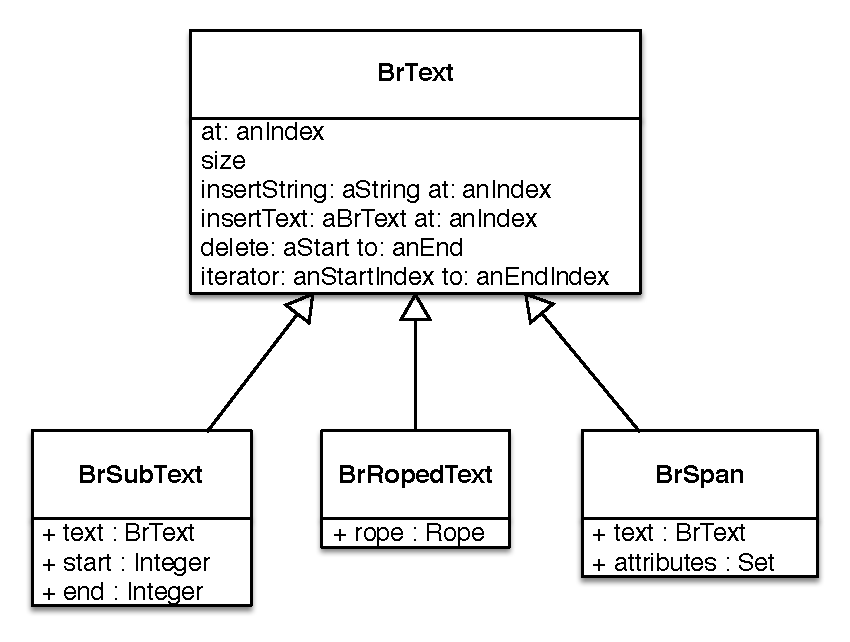
\includegraphics[width=0.65\columnwidth]{figures/text-model-uml.pdf}
\caption{The UML class diagram of Text Model}
\figlabel{TextModelUml}
\end{figure}

In order to display and edit text, an editor requires a text model that provides text modification and enumeration api. In a context of text editor under \textit{Text} we understand an object that consists of a collection of characters with a set of attributes applied on those characters and a number of api methods to support text modifications such as \ct{insert:} or \ct{delete:}. Additionally, text should play a role of sequenceable and indexable collection, allowing uses to iterate over all characters in a natural ordered way. Being indexable is also an essential property of a text model, since text stylers require text to have characters accessible by index. It is a consequence of a fact that code parsers create an \textit{AST} which consists of nodes bound to original text with the help of integer intervals that are later used by a text styler to apply attributes on a piece of text defined by that integer intervals in a form of a \textit{[from, to]} tuple.


\section{Text data structures}

One of the main requirements for the moldable editor is an ability to manipulate large pieces of text that consist of millions of characters and sometimes even more. It means that choosing an appropriate data structure for storing text is crucial. While looking for a data structure that would fit the needs of the moldable editor we found out that there is no the best data structure that is the only choice. It turned out that depending on a context and the way a text editor will be used it may be important to be able to select one or another data structure. Not to mention is the fact that text data structure should be chosen during early development stages, before the editor becomes usable. That is why the text model of the moldable editor is data structure independent and only defines a public api. In order for it to be used by a text editor developers should create concrete implementations of that api with the data structure of choice as a backend. In the following sub-sections we will look at different data structures being used by text editors and compare them.

\subsection{Pharo}

In Pharo there already exist two text models based on different data structures: one is \ct{Text} which is used by both \textit{Morphic} and \textit{Rubric} text editors, and \ct{TxModel} used by \textit{TxText editor}. In the following sections we will compare and evaluate those text models regarding various properties such as ability to store, access and modify large pieces of text or whether they allow developers to embed non-textual object within text.

\subsubsection*{Rubric}

\begin{figure}[ht]
\centering
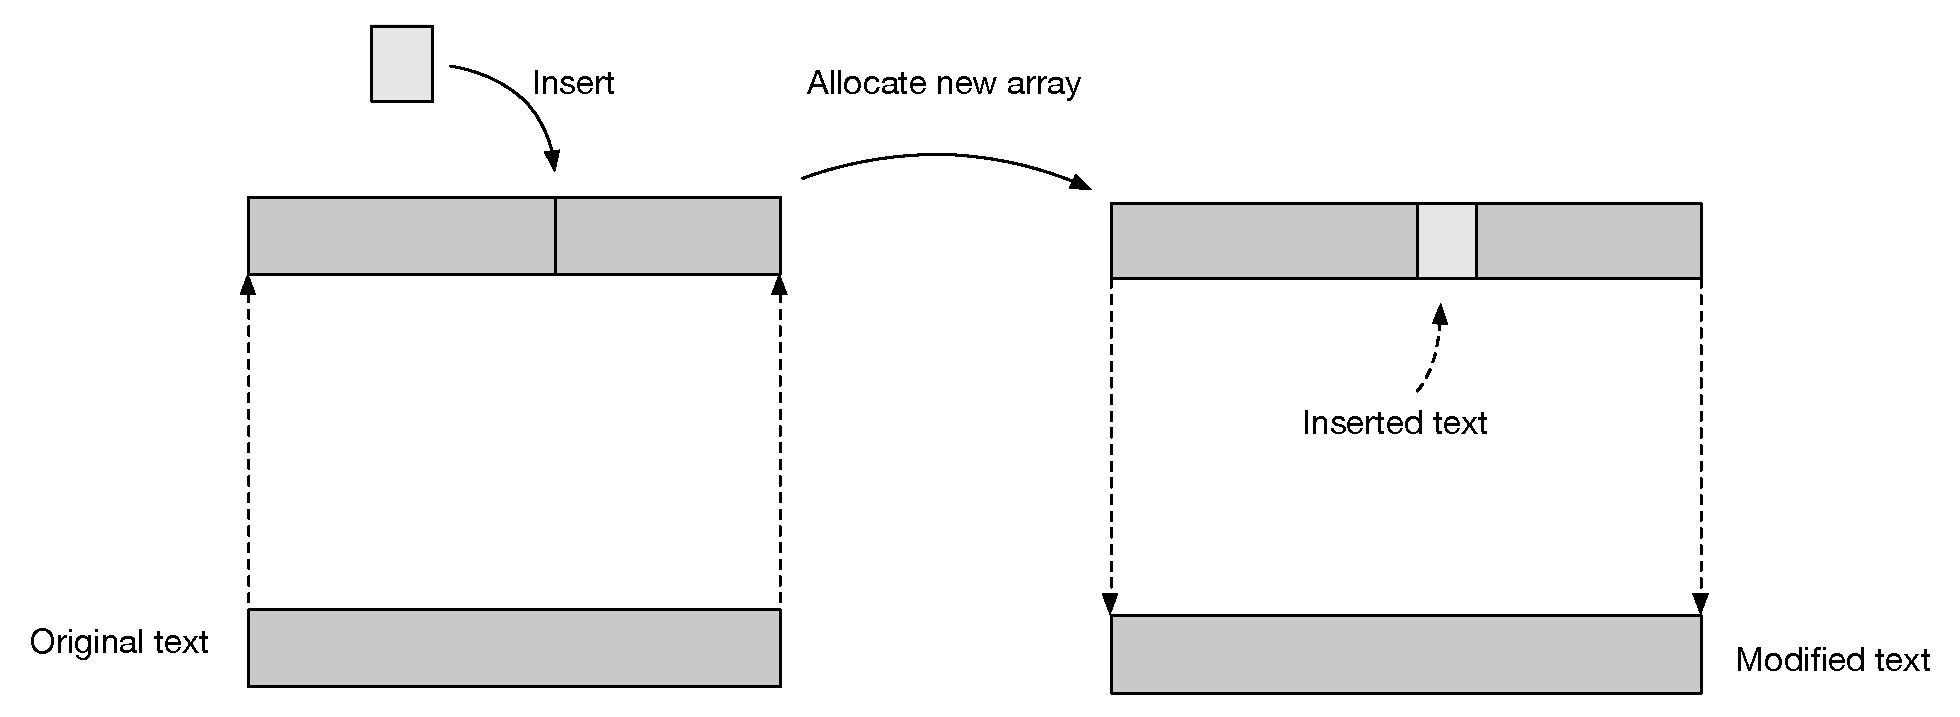
\includegraphics[width=0.85\columnwidth]{figures/data-structure-array.pdf}
\caption{The array method}
\figlabel{ArrayText}
\end{figure}

\code{Text} is a default Pharo text model. It stores a collection of characters and a set of attributes separately. Characters are represented with the help of \ct{ByteString} which is nothing else than an immutable array of characters. It means that every text modification such as insertion or deletion requires text model to allocate and copy the whole array while replacing a subsequence of characters with a requested one as shown on \figref{ArrayText} The algorithm of text modifications is in this case linear time and requires massive memory copy operations, which becomes unacceptably slow when text size growths over hundreds of thousands of characters. In fact, array is the worst data structure for text sequences. \cite{crowley1998data}

\subsubsection*{TxText}

\begin{figure}[ht]
\centering
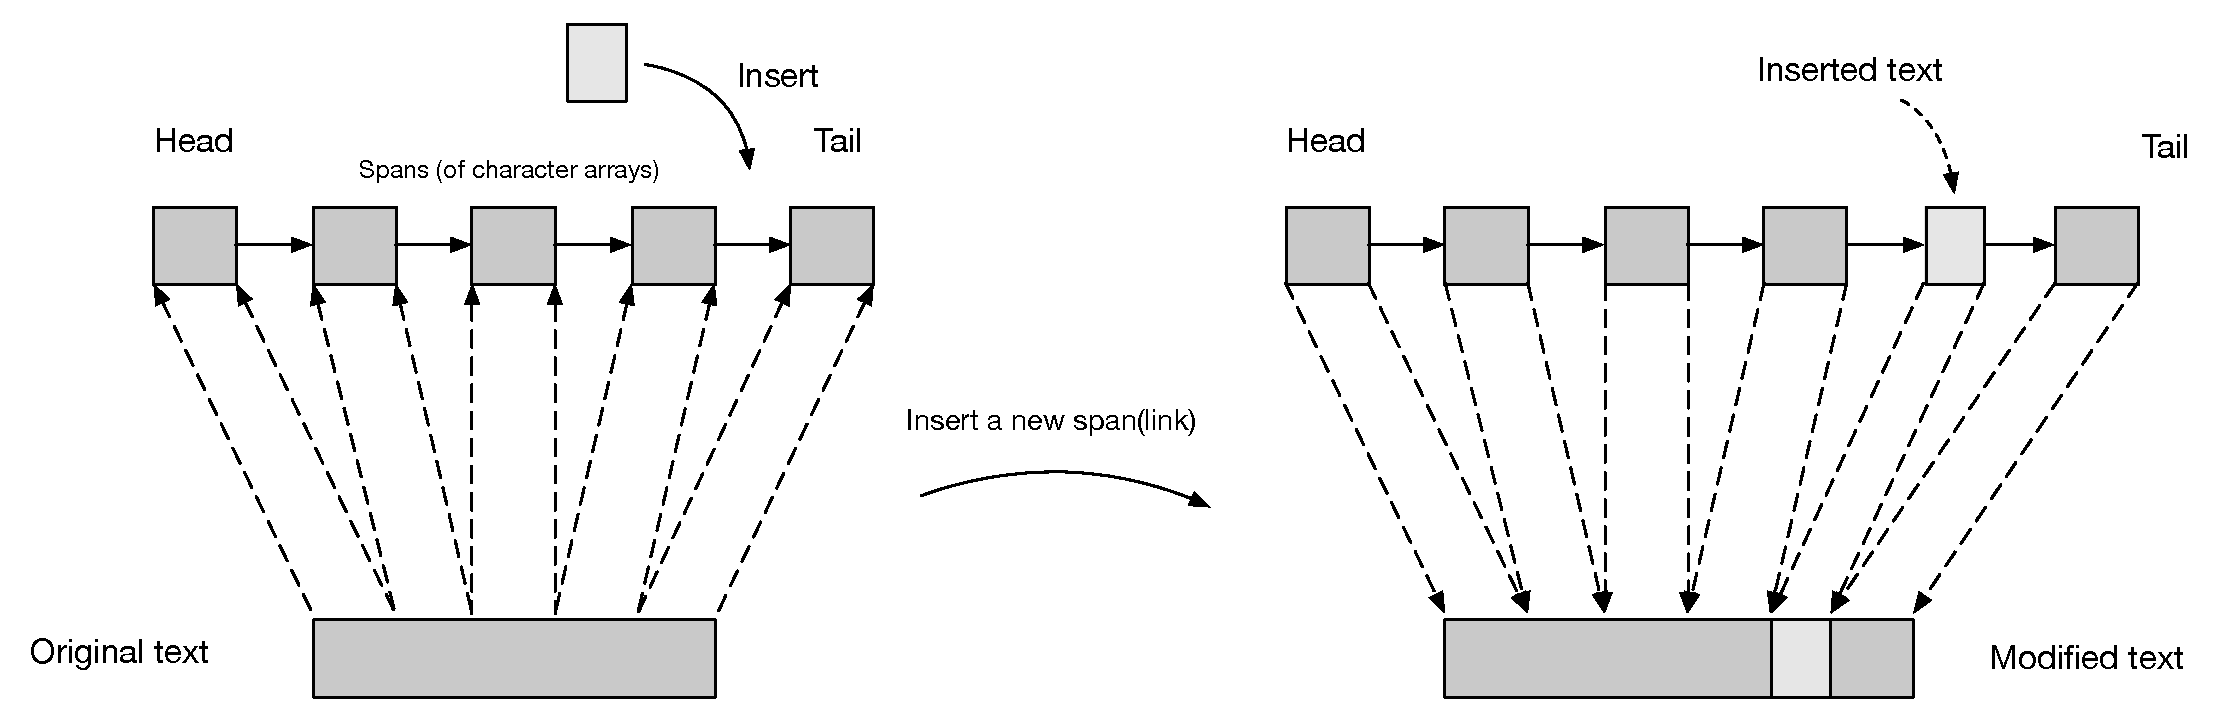
\includegraphics[width=0.85\columnwidth]{figures/data-structure-linked-list.pdf}
\caption{The linked list method}
\figlabel{LinkedListText}
\end{figure}

\code{TxModel} is a central class representing a text in the \textit{TxText editor}. Internally is stores character sequences as a double-linked list of spans that consists of an actual text content. A linked list is considered to be an extreme as opposed to an array method of storing text. While insertions and deletions in a linked list are fast and easy, it is only indexable in a linear time which makes styling one of the slowest among all other text data structures. \cite{crowley1998data}

\subsection{Atom}

Atom text editor uses a memory-efficient data structure similar to a Piece Table.\cite{atomblog2018} Piece table is a memory efficient data structure based of two buffers, one of which represents original read-only text while the second one stores all modifications done to that text. All essential operations are performed with an adequate performance and some of them can  be efficiently improved by using cache. Piece table is considered to be the data structure of choice for a text editor. \cite{crowley1998data}

\subsection{Emacs}

TODO

\subsection{Rope}

TODO


%===================================================================================================
%===================================================================================================
%========================================= A P P L I C A T I O N S ========================================
%===================================================================================================
%===================================================================================================
\chapter {The Validation}


%------------------------------------------------------------------------------------------------------------------------------------------------------------------------------
%--------------------------------------------------------------------------- O V E R V I E W ---------------------------------------------------------------------------%------------------------------------------------------------------------------------------------------------------------------------------------------------------------------

\section{Overview}

\subsection*{Scalability}

The moldable editor is both flexible and scalable. For example, the following piece is a sizeable 2MB of text, and yet it opens smoothly.

%[[[example=BrTextEditorExamples>>#newText|noCode=true|expanded=true|show=gtTextIn:]]]

\subsection*{Syntax highlighting and adornments}

An obvious application for the text editor is a code editor with syntax highlighting.

%[[[example=BrTextEditorExamples>>#elementOnMethodWithSyntaxHighlighting|expanded=true|noCode=true|show=gtLiveIn:]]]

Like in any other text editor that supports syntax highlighting, the syntax highlighter works in a separate process and changes the existing text. Typically, the syntax highlighting affects text attributes such as color or font weight. However, the moldable editor brings this concept further and allows us to add arbitrary visual elements to a text scene.

For example, in the snippet below, we see the code associated with the example that produces the editor element with syntax highlighting seen above. In addition to the typical Pharo syntax highlighting, we can also notice small triangles inserted in the code. These triangles denote a dependency to another example method, and clicking on one expands the code in place showing another editor.

%[[[example=BrTextEditorExamples>>#elementOnMethodWithSyntaxHighlighting|expanded=true|show=gtLiveIn:]]]

This functionality is obtained through a dedicated syntax highlighter that extends the default Pharo highlighting with an extra logic that adds the triangles as adornments. Clicking on such an adornment adds another adornment with another editor element. Interestingly, this all happens live, which means that if you change the code from the root editor element to no longer refer to an example, the corresponding triangle and embedded editor elements will disappear. 

The example above also reveals the way to initialise an editor element.


%------------------------------------------------------------------------------------------------------------------------------------------------------------------------------
%--------------------------------------------------------------------------- T R A N S C R I P T -----------------------------------------------------------------------%------------------------------------------------------------------------------------------------------------------------------------------------------------------------------
\section{Transcript}

Due to its rich abilities, the moldable editor has the potential of changing all tools that rely on textual representations. One such a tool is the Transcript.

In a context Pharo the \textit{Transcript} is a tool that allows users to log stream messages. Additionally, Pharo provides a user interface to show those messages. It means that when it comes to logging tools we should distinguish an API used to output to a stream and a user interface, which is one of the multiple ways to display  the output. Existing \textit{Transcript} in Pharo has an ability to display logged messages in a simple text editor or to write them into a file.


\begin{figure*}[t]
\centering
\subfloat[]{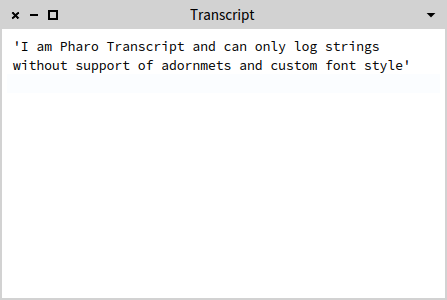
\includegraphics[width=0.32\textwidth]{images/pharo-transcript.png}\figlabel{PharoTranscript}}\hspace{0.1cm}
\subfloat[]{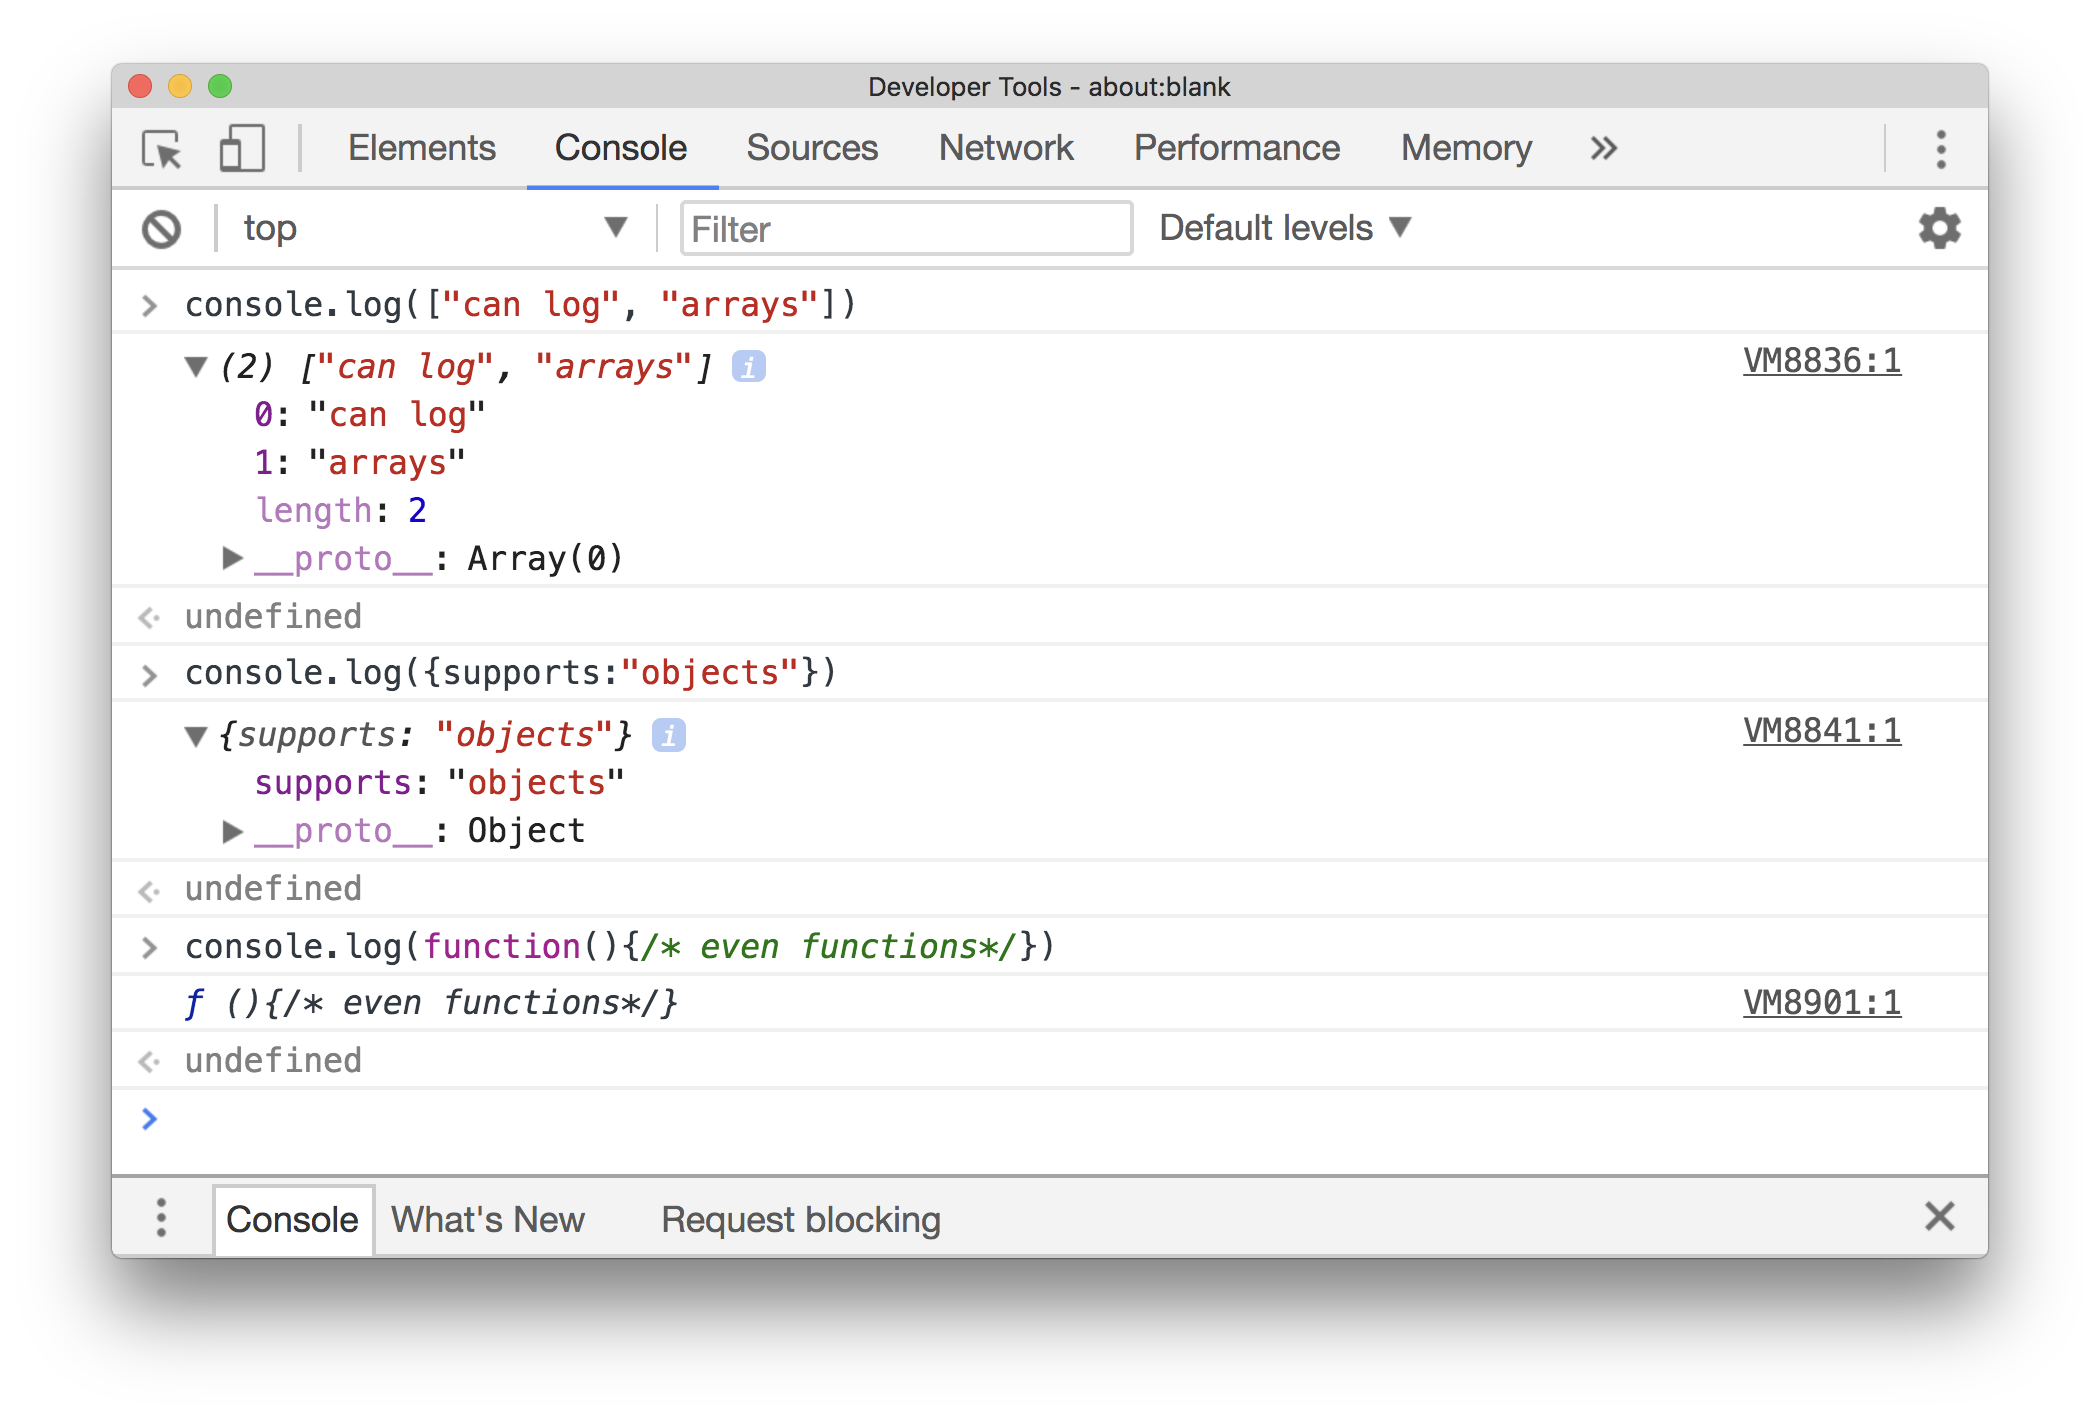
\includegraphics[width=0.32\textwidth]{images/chrome-console.png}\figlabel{ChromeConsole}}\hspace{0.1cm}
\subfloat[]{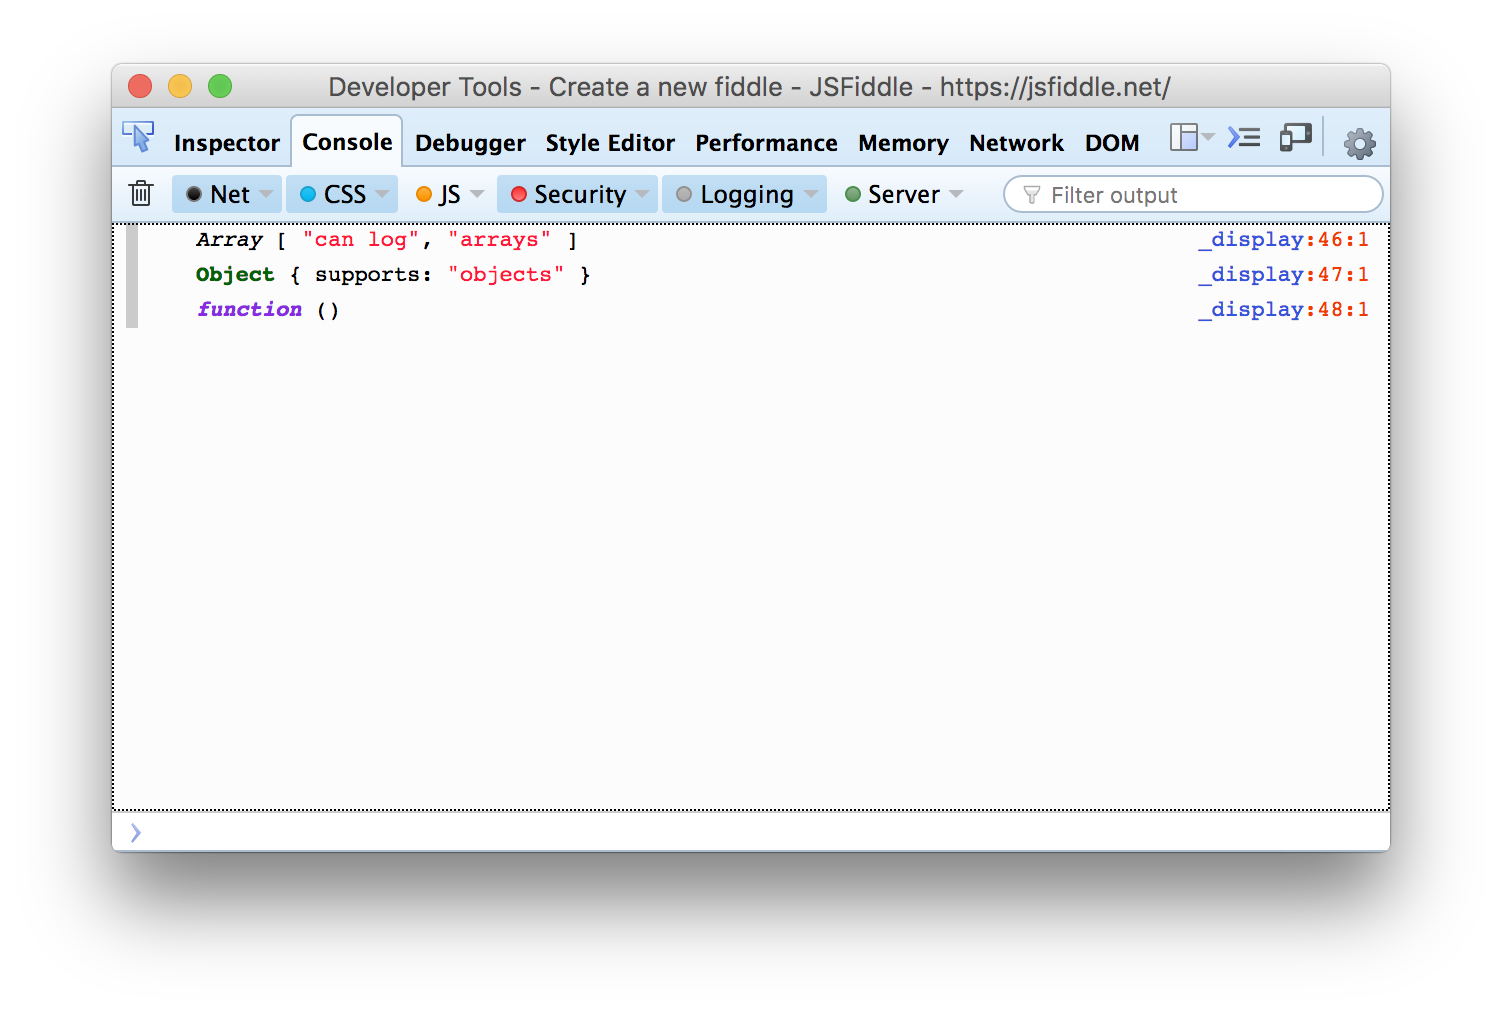
\includegraphics[width=0.32\textwidth]{images/firefox-web-console.png}\figlabel{FirefoxWebConsole}}

\caption{Three different ways to display the code of a method: \emph{a)} the standard Pharo Transcript; \emph{b)} replacing the data parameter using two distinct views; \emph{c)} replacing the results of several intermediary computations.}  
\figlabel{TranscriptTools}
\end{figure*}

Many languages have support of the message logging and their IDEs provide dedicated tools allowing users to browse and read that log. For example in \textit{JavaScript}, the \textit{Console} is an object with an API that can be used to log runtime artefacts such as strings, arrays, functions or object. By default, most modern web browsers are shipped with developer tools and one of them is an interactive console. For example. Mozilla Firefox provides \textit{Web Console} \footnote{\url{https://developer.mozilla.org/en-US/docs/Tools/Web_Console}} which is different from Google Chrome's \textit{Console} \footnote{\url{https://developers.google.com/web/tools/chrome-devtools/console/}} while providing very similar functionality.

The goal of GT Transcript is to offer a rich and interactive interface for displaying live information coming from a system.  

\subsection*{The API}

The API is backward compatible with the existing transcript. To enable the new features, we introduced a builder. For example, \ct{transcript nextPutAll: 'something'} becomes \ct{transcript next putAll: 'something'}. Between \textit{next} and \textit{putAll:}, we can add multiple attributes to the text output.

The following example shows the complete API:

\begin{figure}[t]
\centering
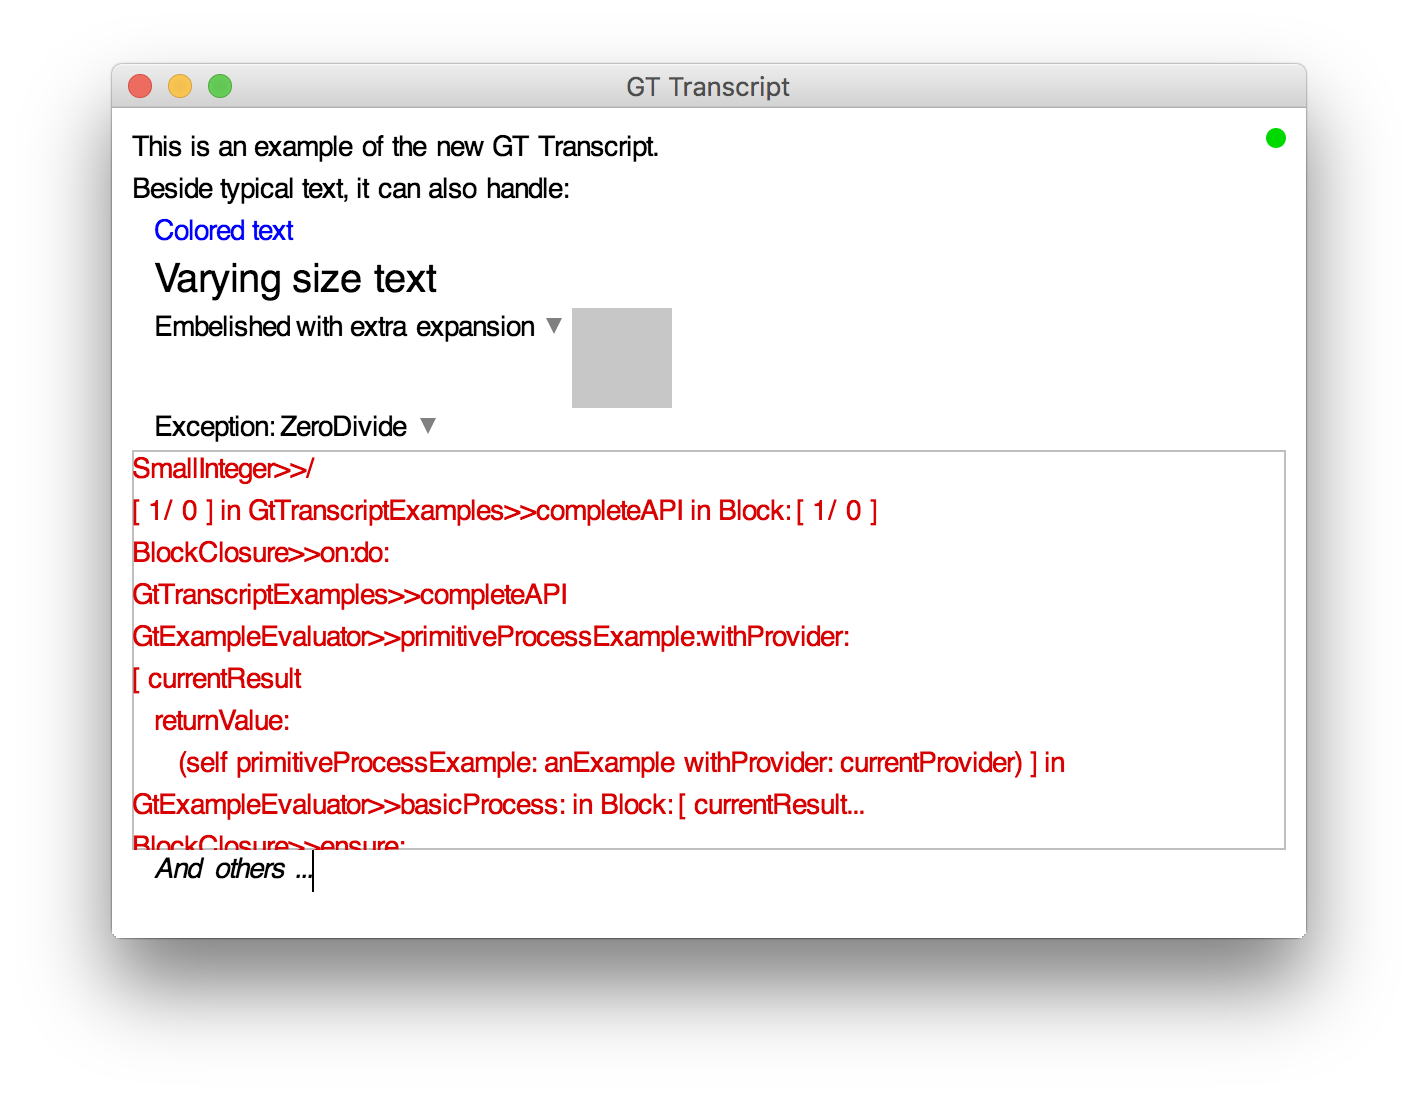
\includegraphics[width=0.85\columnwidth]{images/gt-transcript-complete-api.png}
\caption{Visual output of \lstref{GtTranscriptCompleteApiCode}}
\figlabel{GtTranscriptCompleteApi}
\end{figure}

\begin{minipage}[t]{0.95\textwidth}
\begin{lstlisting}[language=Smalltalk, caption={The complete api of the GT-Transcript},captionpos=b, label={lst:GtTranscriptCompleteApiCode}]
| transcript |
transcript := GtTranscript new.
transcript 
	nextPutAll: 'This is an example of';
	space;
	nextPutAll: 'the new GT Transcript';
	nextPut: '.';
	cr.
transcript next
	putAll: 'Beside typical text, it can also handle:';
	cr.
transcript next
	tab;
	color: Color blue;
	putAll: 'Coloured text';
	cr.
transcript tab.
transcript next	
	fontSize: 20;
	putAll: 'Varying size text';
	cr.
transcript next
	tab;
	expanding: [ BlElement new background: Color gray ];
	putAll: 'Embellished with extra expansion';
	cr.
[ 1/0 ] on: Error do: [ :err | 
	transcript next 
		tab;
		putAll: 'Exception: ';
		showException: err;
		cr ].
transcript next 
	tab;
	italic;
	streamAll: [ transcript next putAll: 'And others ...' ].
\end{lstlisting}

\end{minipage}

\subsection*{Logging an animation}

To get an idea of how this tool could be useful, take a look at the following example. A Bloc animation is logged in a visual, domain centric way, providing insight far superior to plain text.

%[[[example=GtTranscriptExamples>>#transcriptWitAnimation|expanded=true|show=gtLiveIn:]]]

%------------------------------------------------------------------------------------------------------------------------------------------------------------------------------
%--------------------------------------------------------------------------- C O N N E C T O R -----------------------------------------------------------------------%------------------------------------------------------------------------------------------------------------------------------------------------------------------------------
\section{Connector}

In the Overview section, we saw how examples dependencies can be expanded in place by utilizing the syntax highlighter. Connector brings this a step further and proposes a new kind of interface that allows the user to expand a new editor for an example and to automatically connect editor elements with one another.

%[[[example=GtConnectorExamples>>#oneExampleMethod|noCode=true|expanded=true|show=gtLiveIn:]]]

The interface is somewhat similar to the one proposed by Code Bubbles, but it has two key differences:
\begin{itemize}  
\item the lines connect an element inside the text editor to the outside world. This is possible because the text is represented as elements that are rendered in the main rendering tree provided by the underlying Bloc framework.
\item the lines are added automatically to reveal dependencies that are otherwise more difficult to spot.
\end{itemize}

%------------------------------------------------------------------------------------------------------------------------------------------------------------------------------
%-------------------------------------------------------------------------- D O C U M E N T E R ---------------------------------------------------------------------%------------------------------------------------------------------------------------------------------------------------------------------------------------------------------


\section{Documenter}

The Documenter offers live rendering of Pillar documents.


\chapter {Conclusion and Future Work}
In which we step back, have a critical look at the entire work, then conclude, and learn what lays beyond this thesis.

\chapter {Anleitung zu wissenschaftlichen Arbeiten}
This consists of additional documentation, e.g. a tutorial, user guide etc.
Required by the Informatik regulation.

%END Doc
%-------------------------------------------------------

\bibliography{thesis}
\bibliographystyle{plain}

\end{document}